% Created by tikzDevice version 0.12.6 on 2024-07-30 09:43:48
% !TEX encoding = UTF-8 Unicode
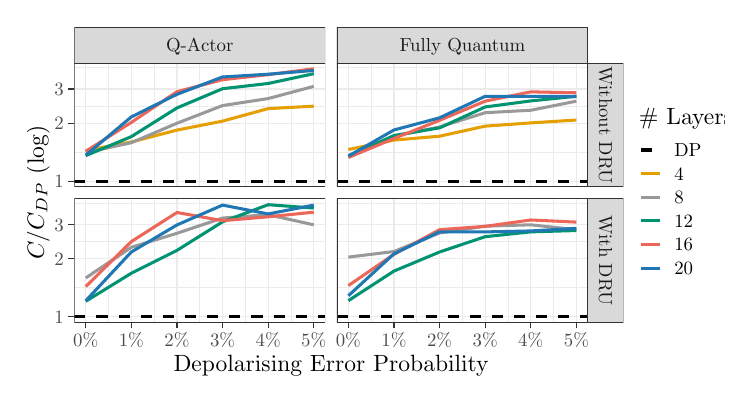
\begin{tikzpicture}[x=1pt,y=1pt]
\definecolor{fillColor}{RGB}{255,255,255}
\path[use as bounding box,fill=fillColor,fill opacity=0.00] (0,0) rectangle (251.96,125.98);
\begin{scope}
\path[clip] (  0.00,  0.00) rectangle (251.96,125.98);
\definecolor{drawColor}{RGB}{255,255,255}
\definecolor{fillColor}{RGB}{255,255,255}

\path[draw=drawColor,line width= 0.4pt,line join=round,line cap=round,fill=fillColor] (  0.00,  0.00) rectangle (251.96,125.98);
\end{scope}
\begin{scope}
\path[clip] ( 16.86, 68.44) rectangle (107.51,113.18);
\definecolor{fillColor}{RGB}{255,255,255}

\path[fill=fillColor] ( 16.86, 68.44) rectangle (107.51,113.18);
\definecolor{drawColor}{gray}{0.92}

\path[draw=drawColor,line width= 0.2pt,line join=round] ( 16.86, 80.99) --
	(107.51, 80.99);

\path[draw=drawColor,line width= 0.2pt,line join=round] ( 16.86, 97.66) --
	(107.51, 97.66);

\path[draw=drawColor,line width= 0.2pt,line join=round] ( 16.86,111.56) --
	(107.51,111.56);

\path[draw=drawColor,line width= 0.2pt,line join=round] ( 29.22, 68.44) --
	( 29.22,113.18);

\path[draw=drawColor,line width= 0.2pt,line join=round] ( 45.70, 68.44) --
	( 45.70,113.18);

\path[draw=drawColor,line width= 0.2pt,line join=round] ( 62.18, 68.44) --
	( 62.18,113.18);

\path[draw=drawColor,line width= 0.2pt,line join=round] ( 78.66, 68.44) --
	( 78.66,113.18);

\path[draw=drawColor,line width= 0.2pt,line join=round] ( 95.14, 68.44) --
	( 95.14,113.18);

\path[draw=drawColor,line width= 0.4pt,line join=round] ( 16.86, 70.48) --
	(107.51, 70.48);

\path[draw=drawColor,line width= 0.4pt,line join=round] ( 16.86, 91.51) --
	(107.51, 91.51);

\path[draw=drawColor,line width= 0.4pt,line join=round] ( 16.86,103.81) --
	(107.51,103.81);

\path[draw=drawColor,line width= 0.4pt,line join=round] ( 20.98, 68.44) --
	( 20.98,113.18);

\path[draw=drawColor,line width= 0.4pt,line join=round] ( 37.46, 68.44) --
	( 37.46,113.18);

\path[draw=drawColor,line width= 0.4pt,line join=round] ( 53.94, 68.44) --
	( 53.94,113.18);

\path[draw=drawColor,line width= 0.4pt,line join=round] ( 70.42, 68.44) --
	( 70.42,113.18);

\path[draw=drawColor,line width= 0.4pt,line join=round] ( 86.90, 68.44) --
	( 86.90,113.18);

\path[draw=drawColor,line width= 0.4pt,line join=round] (103.38, 68.44) --
	(103.38,113.18);
\definecolor{drawColor}{RGB}{230,159,0}

\path[draw=drawColor,line width= 1.1pt,line join=round] ( 20.98, 81.57) --
	( 37.46, 84.68) --
	( 53.94, 88.97) --
	( 70.42, 92.21) --
	( 86.90, 96.73) --
	(103.38, 97.61);
\definecolor{drawColor}{gray}{0.60}

\path[draw=drawColor,line width= 1.1pt,line join=round] ( 20.98, 80.83) --
	( 37.46, 84.41) --
	( 53.94, 91.44) --
	( 70.42, 97.83) --
	( 86.90,100.36) --
	(103.38,104.78);
\definecolor{drawColor}{RGB}{0,147,113}

\path[draw=drawColor,line width= 1.1pt,line join=round] ( 20.98, 79.74) --
	( 37.46, 86.61) --
	( 53.94, 96.97) --
	( 70.42,103.92) --
	( 86.90,105.81) --
	(103.38,109.35);
\definecolor{drawColor}{RGB}{237,102,90}

\path[draw=drawColor,line width= 1.1pt,line join=round] ( 20.98, 81.30) --
	( 37.46, 91.76) --
	( 53.94,102.84) --
	( 70.42,107.18) --
	( 86.90,109.00) --
	(103.38,111.14);
\definecolor{drawColor}{RGB}{31,120,180}

\path[draw=drawColor,line width= 1.1pt,line join=round] ( 20.98, 79.88) --
	( 37.46, 93.74) --
	( 53.94,101.89) --
	( 70.42,108.17) --
	( 86.90,109.16) --
	(103.38,110.51);
\definecolor{drawColor}{RGB}{0,0,0}

\path[draw=drawColor,line width= 1.1pt,dash pattern=on 4pt off 4pt ,line join=round] ( 16.86, 70.48) -- (107.51, 70.48);
\definecolor{drawColor}{gray}{0.20}

\path[draw=drawColor,line width= 0.4pt,line join=round,line cap=round] ( 16.86, 68.44) rectangle (107.51,113.18);
\end{scope}
\begin{scope}
\path[clip] ( 16.86, 19.46) rectangle (107.51, 64.19);
\definecolor{fillColor}{RGB}{255,255,255}

\path[fill=fillColor] ( 16.86, 19.46) rectangle (107.51, 64.19);
\definecolor{drawColor}{gray}{0.92}

\path[draw=drawColor,line width= 0.2pt,line join=round] ( 16.86, 32.01) --
	(107.51, 32.01);

\path[draw=drawColor,line width= 0.2pt,line join=round] ( 16.86, 48.68) --
	(107.51, 48.68);

\path[draw=drawColor,line width= 0.2pt,line join=round] ( 16.86, 62.58) --
	(107.51, 62.58);

\path[draw=drawColor,line width= 0.2pt,line join=round] ( 29.22, 19.46) --
	( 29.22, 64.19);

\path[draw=drawColor,line width= 0.2pt,line join=round] ( 45.70, 19.46) --
	( 45.70, 64.19);

\path[draw=drawColor,line width= 0.2pt,line join=round] ( 62.18, 19.46) --
	( 62.18, 64.19);

\path[draw=drawColor,line width= 0.2pt,line join=round] ( 78.66, 19.46) --
	( 78.66, 64.19);

\path[draw=drawColor,line width= 0.2pt,line join=round] ( 95.14, 19.46) --
	( 95.14, 64.19);

\path[draw=drawColor,line width= 0.4pt,line join=round] ( 16.86, 21.49) --
	(107.51, 21.49);

\path[draw=drawColor,line width= 0.4pt,line join=round] ( 16.86, 42.53) --
	(107.51, 42.53);

\path[draw=drawColor,line width= 0.4pt,line join=round] ( 16.86, 54.83) --
	(107.51, 54.83);

\path[draw=drawColor,line width= 0.4pt,line join=round] ( 20.98, 19.46) --
	( 20.98, 64.19);

\path[draw=drawColor,line width= 0.4pt,line join=round] ( 37.46, 19.46) --
	( 37.46, 64.19);

\path[draw=drawColor,line width= 0.4pt,line join=round] ( 53.94, 19.46) --
	( 53.94, 64.19);

\path[draw=drawColor,line width= 0.4pt,line join=round] ( 70.42, 19.46) --
	( 70.42, 64.19);

\path[draw=drawColor,line width= 0.4pt,line join=round] ( 86.90, 19.46) --
	( 86.90, 64.19);

\path[draw=drawColor,line width= 0.4pt,line join=round] (103.38, 19.46) --
	(103.38, 64.19);
\definecolor{drawColor}{gray}{0.60}

\path[draw=drawColor,line width= 1.1pt,line join=round] ( 20.98, 35.54) --
	( 37.46, 46.61) --
	( 53.94, 51.68) --
	( 70.42, 57.19) --
	( 86.90, 58.41) --
	(103.38, 54.73);
\definecolor{drawColor}{RGB}{0,147,113}

\path[draw=drawColor,line width= 1.1pt,line join=round] ( 20.98, 27.10) --
	( 37.46, 37.25) --
	( 53.94, 45.51) --
	( 70.42, 55.82) --
	( 86.90, 62.01) --
	(103.38, 60.80);
\definecolor{drawColor}{RGB}{237,102,90}

\path[draw=drawColor,line width= 1.1pt,line join=round] ( 20.98, 32.42) --
	( 37.46, 48.68) --
	( 53.94, 59.19) --
	( 70.42, 56.25) --
	( 86.90, 57.64) --
	(103.38, 59.30);
\definecolor{drawColor}{RGB}{31,120,180}

\path[draw=drawColor,line width= 1.1pt,line join=round] ( 20.98, 27.29) --
	( 37.46, 44.93) --
	( 53.94, 54.69) --
	( 70.42, 61.87) --
	( 86.90, 58.67) --
	(103.38, 61.87);
\definecolor{drawColor}{RGB}{0,0,0}

\path[draw=drawColor,line width= 1.1pt,dash pattern=on 4pt off 4pt ,line join=round] ( 16.86, 21.49) -- (107.51, 21.49);
\definecolor{drawColor}{gray}{0.20}

\path[draw=drawColor,line width= 0.4pt,line join=round,line cap=round] ( 16.86, 19.46) rectangle (107.51, 64.19);
\end{scope}
\begin{scope}
\path[clip] (111.76, 68.44) rectangle (202.40,113.18);
\definecolor{fillColor}{RGB}{255,255,255}

\path[fill=fillColor] (111.76, 68.44) rectangle (202.40,113.18);
\definecolor{drawColor}{gray}{0.92}

\path[draw=drawColor,line width= 0.2pt,line join=round] (111.76, 80.99) --
	(202.40, 80.99);

\path[draw=drawColor,line width= 0.2pt,line join=round] (111.76, 97.66) --
	(202.40, 97.66);

\path[draw=drawColor,line width= 0.2pt,line join=round] (111.76,111.56) --
	(202.40,111.56);

\path[draw=drawColor,line width= 0.2pt,line join=round] (124.12, 68.44) --
	(124.12,113.18);

\path[draw=drawColor,line width= 0.2pt,line join=round] (140.60, 68.44) --
	(140.60,113.18);

\path[draw=drawColor,line width= 0.2pt,line join=round] (157.08, 68.44) --
	(157.08,113.18);

\path[draw=drawColor,line width= 0.2pt,line join=round] (173.56, 68.44) --
	(173.56,113.18);

\path[draw=drawColor,line width= 0.2pt,line join=round] (190.04, 68.44) --
	(190.04,113.18);

\path[draw=drawColor,line width= 0.4pt,line join=round] (111.76, 70.48) --
	(202.40, 70.48);

\path[draw=drawColor,line width= 0.4pt,line join=round] (111.76, 91.51) --
	(202.40, 91.51);

\path[draw=drawColor,line width= 0.4pt,line join=round] (111.76,103.81) --
	(202.40,103.81);

\path[draw=drawColor,line width= 0.4pt,line join=round] (115.88, 68.44) --
	(115.88,113.18);

\path[draw=drawColor,line width= 0.4pt,line join=round] (132.36, 68.44) --
	(132.36,113.18);

\path[draw=drawColor,line width= 0.4pt,line join=round] (148.84, 68.44) --
	(148.84,113.18);

\path[draw=drawColor,line width= 0.4pt,line join=round] (165.32, 68.44) --
	(165.32,113.18);

\path[draw=drawColor,line width= 0.4pt,line join=round] (181.80, 68.44) --
	(181.80,113.18);

\path[draw=drawColor,line width= 0.4pt,line join=round] (198.28, 68.44) --
	(198.28,113.18);
\definecolor{drawColor}{RGB}{230,159,0}

\path[draw=drawColor,line width= 1.1pt,line join=round] (115.88, 81.95) --
	(132.36, 85.36) --
	(148.84, 86.76) --
	(165.32, 90.40) --
	(181.80, 91.57) --
	(198.28, 92.61);
\definecolor{drawColor}{gray}{0.60}

\path[draw=drawColor,line width= 1.1pt,line join=round] (115.88, 79.78) --
	(132.36, 86.78) --
	(148.84, 90.11) --
	(165.32, 95.25) --
	(181.80, 96.14) --
	(198.28, 99.43);
\definecolor{drawColor}{RGB}{0,147,113}

\path[draw=drawColor,line width= 1.1pt,line join=round] (115.88, 79.51) --
	(132.36, 87.00) --
	(148.84, 89.77) --
	(165.32, 97.33) --
	(181.80, 99.51) --
	(198.28,101.19);
\definecolor{drawColor}{RGB}{237,102,90}

\path[draw=drawColor,line width= 1.1pt,line join=round] (115.88, 79.06) --
	(132.36, 85.94) --
	(148.84, 92.50) --
	(165.32, 99.43) --
	(181.80,102.79) --
	(198.28,102.45);
\definecolor{drawColor}{RGB}{31,120,180}

\path[draw=drawColor,line width= 1.1pt,line join=round] (115.88, 79.56) --
	(132.36, 89.01) --
	(148.84, 93.40) --
	(165.32,101.19) --
	(181.80,101.19) --
	(198.28,101.10);
\definecolor{drawColor}{RGB}{0,0,0}

\path[draw=drawColor,line width= 1.1pt,dash pattern=on 4pt off 4pt ,line join=round] (111.76, 70.48) -- (202.40, 70.48);
\definecolor{drawColor}{gray}{0.20}

\path[draw=drawColor,line width= 0.4pt,line join=round,line cap=round] (111.76, 68.44) rectangle (202.40,113.18);
\end{scope}
\begin{scope}
\path[clip] (111.76, 19.46) rectangle (202.40, 64.19);
\definecolor{fillColor}{RGB}{255,255,255}

\path[fill=fillColor] (111.76, 19.46) rectangle (202.40, 64.19);
\definecolor{drawColor}{gray}{0.92}

\path[draw=drawColor,line width= 0.2pt,line join=round] (111.76, 32.01) --
	(202.40, 32.01);

\path[draw=drawColor,line width= 0.2pt,line join=round] (111.76, 48.68) --
	(202.40, 48.68);

\path[draw=drawColor,line width= 0.2pt,line join=round] (111.76, 62.58) --
	(202.40, 62.58);

\path[draw=drawColor,line width= 0.2pt,line join=round] (124.12, 19.46) --
	(124.12, 64.19);

\path[draw=drawColor,line width= 0.2pt,line join=round] (140.60, 19.46) --
	(140.60, 64.19);

\path[draw=drawColor,line width= 0.2pt,line join=round] (157.08, 19.46) --
	(157.08, 64.19);

\path[draw=drawColor,line width= 0.2pt,line join=round] (173.56, 19.46) --
	(173.56, 64.19);

\path[draw=drawColor,line width= 0.2pt,line join=round] (190.04, 19.46) --
	(190.04, 64.19);

\path[draw=drawColor,line width= 0.4pt,line join=round] (111.76, 21.49) --
	(202.40, 21.49);

\path[draw=drawColor,line width= 0.4pt,line join=round] (111.76, 42.53) --
	(202.40, 42.53);

\path[draw=drawColor,line width= 0.4pt,line join=round] (111.76, 54.83) --
	(202.40, 54.83);

\path[draw=drawColor,line width= 0.4pt,line join=round] (115.88, 19.46) --
	(115.88, 64.19);

\path[draw=drawColor,line width= 0.4pt,line join=round] (132.36, 19.46) --
	(132.36, 64.19);

\path[draw=drawColor,line width= 0.4pt,line join=round] (148.84, 19.46) --
	(148.84, 64.19);

\path[draw=drawColor,line width= 0.4pt,line join=round] (165.32, 19.46) --
	(165.32, 64.19);

\path[draw=drawColor,line width= 0.4pt,line join=round] (181.80, 19.46) --
	(181.80, 64.19);

\path[draw=drawColor,line width= 0.4pt,line join=round] (198.28, 19.46) --
	(198.28, 64.19);
\definecolor{drawColor}{gray}{0.60}

\path[draw=drawColor,line width= 1.1pt,line join=round] (115.88, 43.07) --
	(132.36, 45.09) --
	(148.84, 51.78) --
	(165.32, 54.25) --
	(181.80, 54.75) --
	(198.28, 52.98);
\definecolor{drawColor}{RGB}{0,147,113}

\path[draw=drawColor,line width= 1.1pt,line join=round] (115.88, 27.34) --
	(132.36, 38.02) --
	(148.84, 44.92) --
	(165.32, 50.45) --
	(181.80, 52.19) --
	(198.28, 52.68);
\definecolor{drawColor}{RGB}{237,102,90}

\path[draw=drawColor,line width= 1.1pt,line join=round] (115.88, 32.78) --
	(132.36, 44.07) --
	(148.84, 52.98) --
	(165.32, 54.19) --
	(181.80, 56.49) --
	(198.28, 55.72);
\definecolor{drawColor}{RGB}{31,120,180}

\path[draw=drawColor,line width= 1.1pt,line join=round] (115.88, 29.11) --
	(132.36, 44.27) --
	(148.84, 52.21) --
	(165.32, 52.18) --
	(181.80, 52.53) --
	(198.28, 53.47);
\definecolor{drawColor}{RGB}{0,0,0}

\path[draw=drawColor,line width= 1.1pt,dash pattern=on 4pt off 4pt ,line join=round] (111.76, 21.49) -- (202.40, 21.49);
\definecolor{drawColor}{gray}{0.20}

\path[draw=drawColor,line width= 0.4pt,line join=round,line cap=round] (111.76, 19.46) rectangle (202.40, 64.19);
\end{scope}
\begin{scope}
\path[clip] ( 16.86,113.18) rectangle (107.51,125.98);
\definecolor{drawColor}{gray}{0.20}
\definecolor{fillColor}{gray}{0.85}

\path[draw=drawColor,line width= 0.4pt,line join=round,line cap=round,fill=fillColor] ( 16.86,113.18) rectangle (107.51,125.98);
\definecolor{drawColor}{gray}{0.10}

\node[text=drawColor,anchor=base,inner sep=0pt, outer sep=0pt, scale=  0.68] at ( 62.18,117.24) {Q-Actor};
\end{scope}
\begin{scope}
\path[clip] (111.76,113.18) rectangle (202.40,125.98);
\definecolor{drawColor}{gray}{0.20}
\definecolor{fillColor}{gray}{0.85}

\path[draw=drawColor,line width= 0.4pt,line join=round,line cap=round,fill=fillColor] (111.76,113.18) rectangle (202.40,125.98);
\definecolor{drawColor}{gray}{0.10}

\node[text=drawColor,anchor=base,inner sep=0pt, outer sep=0pt, scale=  0.68] at (157.08,117.24) {Fully Quantum};
\end{scope}
\begin{scope}
\path[clip] (202.40, 68.44) rectangle (215.21,113.18);
\definecolor{drawColor}{gray}{0.20}
\definecolor{fillColor}{gray}{0.85}

\path[draw=drawColor,line width= 0.4pt,line join=round,line cap=round,fill=fillColor] (202.40, 68.44) rectangle (215.21,113.18);
\definecolor{drawColor}{gray}{0.10}

\node[text=drawColor,rotate=-90.00,anchor=base,inner sep=0pt, outer sep=0pt, scale=  0.68] at (206.47, 90.81) {Without DRU};
\end{scope}
\begin{scope}
\path[clip] (202.40, 19.46) rectangle (215.21, 64.19);
\definecolor{drawColor}{gray}{0.20}
\definecolor{fillColor}{gray}{0.85}

\path[draw=drawColor,line width= 0.4pt,line join=round,line cap=round,fill=fillColor] (202.40, 19.46) rectangle (215.21, 64.19);
\definecolor{drawColor}{gray}{0.10}

\node[text=drawColor,rotate=-90.00,anchor=base,inner sep=0pt, outer sep=0pt, scale=  0.68] at (206.47, 41.83) {With DRU};
\end{scope}
\begin{scope}
\path[clip] (  0.00,  0.00) rectangle (251.96,125.98);
\definecolor{drawColor}{gray}{0.20}

\path[draw=drawColor,line width= 0.4pt,line join=round] ( 20.98, 17.34) --
	( 20.98, 19.46);

\path[draw=drawColor,line width= 0.4pt,line join=round] ( 37.46, 17.34) --
	( 37.46, 19.46);

\path[draw=drawColor,line width= 0.4pt,line join=round] ( 53.94, 17.34) --
	( 53.94, 19.46);

\path[draw=drawColor,line width= 0.4pt,line join=round] ( 70.42, 17.34) --
	( 70.42, 19.46);

\path[draw=drawColor,line width= 0.4pt,line join=round] ( 86.90, 17.34) --
	( 86.90, 19.46);

\path[draw=drawColor,line width= 0.4pt,line join=round] (103.38, 17.34) --
	(103.38, 19.46);
\end{scope}
\begin{scope}
\path[clip] (  0.00,  0.00) rectangle (251.96,125.98);
\definecolor{drawColor}{gray}{0.30}

\node[text=drawColor,anchor=base,inner sep=0pt, outer sep=0pt, scale=  0.68] at ( 20.98, 10.95) {0\%};

\node[text=drawColor,anchor=base,inner sep=0pt, outer sep=0pt, scale=  0.68] at ( 37.46, 10.95) {1\%};

\node[text=drawColor,anchor=base,inner sep=0pt, outer sep=0pt, scale=  0.68] at ( 53.94, 10.95) {2\%};

\node[text=drawColor,anchor=base,inner sep=0pt, outer sep=0pt, scale=  0.68] at ( 70.42, 10.95) {3\%};

\node[text=drawColor,anchor=base,inner sep=0pt, outer sep=0pt, scale=  0.68] at ( 86.90, 10.95) {4\%};

\node[text=drawColor,anchor=base,inner sep=0pt, outer sep=0pt, scale=  0.68] at (103.38, 10.95) {5\%};
\end{scope}
\begin{scope}
\path[clip] (  0.00,  0.00) rectangle (251.96,125.98);
\definecolor{drawColor}{gray}{0.20}

\path[draw=drawColor,line width= 0.4pt,line join=round] (115.88, 17.34) --
	(115.88, 19.46);

\path[draw=drawColor,line width= 0.4pt,line join=round] (132.36, 17.34) --
	(132.36, 19.46);

\path[draw=drawColor,line width= 0.4pt,line join=round] (148.84, 17.34) --
	(148.84, 19.46);

\path[draw=drawColor,line width= 0.4pt,line join=round] (165.32, 17.34) --
	(165.32, 19.46);

\path[draw=drawColor,line width= 0.4pt,line join=round] (181.80, 17.34) --
	(181.80, 19.46);

\path[draw=drawColor,line width= 0.4pt,line join=round] (198.28, 17.34) --
	(198.28, 19.46);
\end{scope}
\begin{scope}
\path[clip] (  0.00,  0.00) rectangle (251.96,125.98);
\definecolor{drawColor}{gray}{0.30}

\node[text=drawColor,anchor=base,inner sep=0pt, outer sep=0pt, scale=  0.68] at (115.88, 10.95) {0\%};

\node[text=drawColor,anchor=base,inner sep=0pt, outer sep=0pt, scale=  0.68] at (132.36, 10.95) {1\%};

\node[text=drawColor,anchor=base,inner sep=0pt, outer sep=0pt, scale=  0.68] at (148.84, 10.95) {2\%};

\node[text=drawColor,anchor=base,inner sep=0pt, outer sep=0pt, scale=  0.68] at (165.32, 10.95) {3\%};

\node[text=drawColor,anchor=base,inner sep=0pt, outer sep=0pt, scale=  0.68] at (181.80, 10.95) {4\%};

\node[text=drawColor,anchor=base,inner sep=0pt, outer sep=0pt, scale=  0.68] at (198.28, 10.95) {5\%};
\end{scope}
\begin{scope}
\path[clip] (  0.00,  0.00) rectangle (251.96,125.98);
\definecolor{drawColor}{gray}{0.30}

\node[text=drawColor,anchor=base east,inner sep=0pt, outer sep=0pt, scale=  0.68] at ( 13.03, 68.14) {1};

\node[text=drawColor,anchor=base east,inner sep=0pt, outer sep=0pt, scale=  0.68] at ( 13.03, 89.17) {2};

\node[text=drawColor,anchor=base east,inner sep=0pt, outer sep=0pt, scale=  0.68] at ( 13.03,101.47) {3};
\end{scope}
\begin{scope}
\path[clip] (  0.00,  0.00) rectangle (251.96,125.98);
\definecolor{drawColor}{gray}{0.20}

\path[draw=drawColor,line width= 0.4pt,line join=round] ( 14.73, 70.48) --
	( 16.86, 70.48);

\path[draw=drawColor,line width= 0.4pt,line join=round] ( 14.73, 91.51) --
	( 16.86, 91.51);

\path[draw=drawColor,line width= 0.4pt,line join=round] ( 14.73,103.81) --
	( 16.86,103.81);
\end{scope}
\begin{scope}
\path[clip] (  0.00,  0.00) rectangle (251.96,125.98);
\definecolor{drawColor}{gray}{0.30}

\node[text=drawColor,anchor=base east,inner sep=0pt, outer sep=0pt, scale=  0.68] at ( 13.03, 19.15) {1};

\node[text=drawColor,anchor=base east,inner sep=0pt, outer sep=0pt, scale=  0.68] at ( 13.03, 40.19) {2};

\node[text=drawColor,anchor=base east,inner sep=0pt, outer sep=0pt, scale=  0.68] at ( 13.03, 52.49) {3};
\end{scope}
\begin{scope}
\path[clip] (  0.00,  0.00) rectangle (251.96,125.98);
\definecolor{drawColor}{gray}{0.20}

\path[draw=drawColor,line width= 0.4pt,line join=round] ( 14.73, 21.49) --
	( 16.86, 21.49);

\path[draw=drawColor,line width= 0.4pt,line join=round] ( 14.73, 42.53) --
	( 16.86, 42.53);

\path[draw=drawColor,line width= 0.4pt,line join=round] ( 14.73, 54.83) --
	( 16.86, 54.83);
\end{scope}
\begin{scope}
\path[clip] (  0.00,  0.00) rectangle (251.96,125.98);
\definecolor{drawColor}{RGB}{0,0,0}

\node[text=drawColor,anchor=base,inner sep=0pt, outer sep=0pt, scale=  0.85] at (109.63,  1.65) {Depolarising Error Probability};
\end{scope}
\begin{scope}
\path[clip] (  0.00,  0.00) rectangle (251.96,125.98);
\definecolor{drawColor}{RGB}{0,0,0}

\node[text=drawColor,rotate= 90.00,anchor=base,inner sep=0pt, outer sep=0pt, scale=  0.85] at (  5.85, 66.32) {$C/C_{\text{DP}}$ (log)};
\end{scope}
\begin{scope}
\path[clip] (  0.00,  0.00) rectangle (251.96,125.98);
\definecolor{fillColor}{RGB}{255,255,255}

\path[fill=fillColor] (223.71, 34.83) rectangle (251.96, 97.81);
\end{scope}
\begin{scope}
\path[clip] (  0.00,  0.00) rectangle (251.96,125.98);
\definecolor{drawColor}{RGB}{0,0,0}

\node[text=drawColor,anchor=base west,inner sep=0pt, outer sep=0pt, scale=  0.85] at (220.86, 91.12) {\# Layers};
\end{scope}
\begin{scope}
\path[clip] (  0.00,  0.00) rectangle (251.96,125.98);
\definecolor{fillColor}{RGB}{255,255,255}

\path[fill=fillColor] (220.86, 77.51) rectangle (229.40, 86.05);
\end{scope}
\begin{scope}
\path[clip] (  0.00,  0.00) rectangle (251.96,125.98);
\definecolor{drawColor}{RGB}{0,0,0}

\path[draw=drawColor,line width= 1.1pt,dash pattern=on 4pt off 4pt ,line join=round] (221.72, 81.78) -- (228.55, 81.78);
\end{scope}
\begin{scope}
\path[clip] (  0.00,  0.00) rectangle (251.96,125.98);
\definecolor{fillColor}{RGB}{255,255,255}

\path[fill=fillColor] (220.86, 68.98) rectangle (229.40, 77.51);
\end{scope}
\begin{scope}
\path[clip] (  0.00,  0.00) rectangle (251.96,125.98);
\definecolor{drawColor}{RGB}{230,159,0}

\path[draw=drawColor,line width= 1.1pt,line join=round] (221.72, 73.24) -- (228.55, 73.24);
\end{scope}
\begin{scope}
\path[clip] (  0.00,  0.00) rectangle (251.96,125.98);
\definecolor{fillColor}{RGB}{255,255,255}

\path[fill=fillColor] (220.86, 60.44) rectangle (229.40, 68.98);
\end{scope}
\begin{scope}
\path[clip] (  0.00,  0.00) rectangle (251.96,125.98);
\definecolor{drawColor}{gray}{0.60}

\path[draw=drawColor,line width= 1.1pt,line join=round] (221.72, 64.71) -- (228.55, 64.71);
\end{scope}
\begin{scope}
\path[clip] (  0.00,  0.00) rectangle (251.96,125.98);
\definecolor{fillColor}{RGB}{255,255,255}

\path[fill=fillColor] (220.86, 51.91) rectangle (229.40, 60.44);
\end{scope}
\begin{scope}
\path[clip] (  0.00,  0.00) rectangle (251.96,125.98);
\definecolor{drawColor}{RGB}{0,147,113}

\path[draw=drawColor,line width= 1.1pt,line join=round] (221.72, 56.17) -- (228.55, 56.17);
\end{scope}
\begin{scope}
\path[clip] (  0.00,  0.00) rectangle (251.96,125.98);
\definecolor{fillColor}{RGB}{255,255,255}

\path[fill=fillColor] (220.86, 43.37) rectangle (229.40, 51.91);
\end{scope}
\begin{scope}
\path[clip] (  0.00,  0.00) rectangle (251.96,125.98);
\definecolor{drawColor}{RGB}{237,102,90}

\path[draw=drawColor,line width= 1.1pt,line join=round] (221.72, 47.64) -- (228.55, 47.64);
\end{scope}
\begin{scope}
\path[clip] (  0.00,  0.00) rectangle (251.96,125.98);
\definecolor{fillColor}{RGB}{255,255,255}

\path[fill=fillColor] (220.86, 34.83) rectangle (229.40, 43.37);
\end{scope}
\begin{scope}
\path[clip] (  0.00,  0.00) rectangle (251.96,125.98);
\definecolor{drawColor}{RGB}{31,120,180}

\path[draw=drawColor,line width= 1.1pt,line join=round] (221.72, 39.10) -- (228.55, 39.10);
\end{scope}
\begin{scope}
\path[clip] (  0.00,  0.00) rectangle (251.96,125.98);
\definecolor{drawColor}{RGB}{0,0,0}

\node[text=drawColor,anchor=base west,inner sep=0pt, outer sep=0pt, scale=  0.68] at (233.65, 79.44) {DP};
\end{scope}
\begin{scope}
\path[clip] (  0.00,  0.00) rectangle (251.96,125.98);
\definecolor{drawColor}{RGB}{0,0,0}

\node[text=drawColor,anchor=base west,inner sep=0pt, outer sep=0pt, scale=  0.68] at (233.65, 70.90) {4};
\end{scope}
\begin{scope}
\path[clip] (  0.00,  0.00) rectangle (251.96,125.98);
\definecolor{drawColor}{RGB}{0,0,0}

\node[text=drawColor,anchor=base west,inner sep=0pt, outer sep=0pt, scale=  0.68] at (233.65, 62.37) {8};
\end{scope}
\begin{scope}
\path[clip] (  0.00,  0.00) rectangle (251.96,125.98);
\definecolor{drawColor}{RGB}{0,0,0}

\node[text=drawColor,anchor=base west,inner sep=0pt, outer sep=0pt, scale=  0.68] at (233.65, 53.83) {12};
\end{scope}
\begin{scope}
\path[clip] (  0.00,  0.00) rectangle (251.96,125.98);
\definecolor{drawColor}{RGB}{0,0,0}

\node[text=drawColor,anchor=base west,inner sep=0pt, outer sep=0pt, scale=  0.68] at (233.65, 45.30) {16};
\end{scope}
\begin{scope}
\path[clip] (  0.00,  0.00) rectangle (251.96,125.98);
\definecolor{drawColor}{RGB}{0,0,0}

\node[text=drawColor,anchor=base west,inner sep=0pt, outer sep=0pt, scale=  0.68] at (233.65, 36.76) {20};
\end{scope}
\end{tikzpicture}
